%-*- coding:utf-8 -*-

\documentclass[10pt,dvipdfmx]{beamer}
\usepackage{tutorial}

\title{計算機実験II (L2) \\ マルコフ連鎖モンテカルロ}
\date{2020/10/02}

\begin{document}

\begin{frame}
  \titlepage
  \tableofcontents
\end{frame}

\begin{frame}[t]{講義日程}
  \begin{itemize}
    % \setlength{\itemsep}{1em}
  \item 全8回 (金曜5限 {\color{red}17:05}-18:35)
    \begin{itemize}
    \item {\color{gray} 10月8日 第1回: 乱択アルゴリズム、モンテカルロ法}
    \item 10月15日 第2回: 多体系の統計力学、マルコフ連鎖モンテカルロ法
    \item 10月22日 第3回
    \item 10月29日 第4回
    \item 11月5日 休講 (もくもく会)
    \item 11月12日 休講 (物理学教室コロキウム)
    \item 11月19日 第5回
    \item 11月26日 休講 (物理学教室コロキウム)
    \item 12月3日 第6回
    \item 12月10日 第7回
    \item 12月17日 休講 (物理学教室コロキウム)
    \item 12月24日 第8回
    \item 1月7日 休講 (もくもく会)
    \item 1月18日(火) 休講 (予備日)
    \end{itemize}
  \end{itemize}
\end{frame}


\section{多体系の統計力学}

\begin{frame}[t,fragile]{典型的な統計力学モデル}
  \begin{itemize}
    %\setlength{\itemsep}{1em}
  \item 古典粒子系
    \begin{itemize}
    \item 調和振動子 \ \ $\displaystyle H = \frac{p^2}{2m} + \frac{k}{2}x^2$
    \item 多粒子系
      \[
      H = \sum \frac{p_i^2}{2m} + \sum_{ij} V(x_i, x_j)
      \]
    \item バネビーズ模型
      \[
      H = \sum \frac{p_i^2}{2m} + \frac{k}{2} \sum_{ij} (x_i-x_j)^2
      \]
  \end{itemize}
  \item 磁性体
    \begin{itemize}
    \item イジング模型 \ \ $\displaystyle H = -J \sum_{ij} \sigma_i \sigma_j$ \ \ \ $\sigma_i = \pm 1$
    \end{itemize}
  \end{itemize}
\end{frame}

%-*- coding:utf-8 -*-

\begin{frame}[t,fragile]{多体系の統計力学}
  \begin{itemize}
    %\setlength{\itemsep}{1em}
  \item カノニカル分布 \ $\pi(s) = \exp [- \beta H(s) ] / Z$ \ \ \ ($\beta = k_{\rm B} T$)
  \item 分配関数・自由エネルギー
    \begin{align*}
      Z(T) &= \int \exp [- \beta H(p,x) ] \, dp \, dx \qquad \text{(連続変数)} \\
      &= \sum_s \exp [- \beta H(s) ] \qquad \text{(離散変数)} \\
      f(T) &= - \beta^{-1} \log Z(T)
    \end{align*}
  \item 物理量の期待値
    \begin{align*}
      \langle A \rangle &= Z^{-1} \int A(p,x) \exp [- \beta H(p,x) ] \, dp \, dx \qquad \text{(連続変数)} \\
      &= Z^{-1} \sum_s A(s) \exp [- \beta H(s) ] \qquad \text{(離散変数)}
    \end{align*}
  \end{itemize}
\end{frame}

%-*- coding:utf-8 -*-

\begin{frame}[t,fragile]{多体系の統計力学}
  \begin{itemize}
    % \setlength{\itemsep}{1em}
  \item 内部エネルギー
    \begin{align*}
      E &= -\frac{\partial}{\partial\beta} \log Z = Z^{-1} \sum_s H(s) \exp [- \beta H(s) ] = \langle H \rangle
    \end{align*}
  \item 比熱
    \begin{align*}
      C &= \frac{1}{N} \frac{\partial E}{\partial T} = \frac{\beta^2}{N} (\langle H^2 \rangle - \langle H \rangle^2)
    \end{align*}
  \end{itemize}
\end{frame}

%-*- coding:utf-8 -*-

\begin{frame}[t,fragile]{様々な数値計算手法}
  \begin{itemize}
    % \setlength{\itemsep}{1em}
  \item 数え上げ (離散変数)
    \begin{itemize}
      \item 計算コスト × (指数関数的)
      \item メモリコスト ○ (${\cal O}(1)$)
    \end{itemize}
  \item 転送行列法 (離散変数)
    \begin{itemize}
      \item 計算コスト △ (指数関数的)
      \item メモリコスト △ (指数関数的)
    \end{itemize}
  \item 分子動力学法 (連続変数)
    \begin{itemize}
      \item 計算コスト ○ (${\cal O}(N)$)
      \item メモリコスト ○ (${\cal O}(N)$)
      \item 統計誤差あり
    \end{itemize}
  \item マルコフ連鎖モンテカルロ法 (離散変数・連続変数)
    \begin{itemize}
      \item 計算コスト ○ (${\cal O}(N)$)
      \item メモリコスト ○ (${\cal O}(N)$)
      \item 統計誤差あり
    \end{itemize}
  \end{itemize}
\end{frame}


\section{数え上げ}

%-*- coding:utf-8 -*-

\begin{frame}[t,fragile]{厳密な数え上げ}
  \begin{itemize}
    %\setlength{\itemsep}{1em}
  \item 全ての状態についてボルツマン重みを計算し足し合わせる
    \begin{itemize}
    \item 状態数 $= 2^N$ \ ($N$スピン数)
    \end{itemize}
  \item $N$重のforループを書く代わりに、状態を{\color{red}$N$ビットの整数}($s=0,\cdots,2^N-1$)で表し一つのループに
    \begin{itemize}
    \item $i$番目($i=0,\cdots,N-1$)の格子点のスピンの状態を$i$ビット目に保存
    \item $\sigma = \pm 1$をビットの 1 or 0で表現
    \item シフト演算(\verb+>>+)とAND演算(\verb+&+)でスピン状態を取り出す

      例: 4番目($i=3$)のビットを取り出す: \verb+(s>>3)&1+

      例: $\sigma_i \sigma_j$の計算: \verb+(2.0*((s>>i)&1)-1)*(2.0*((s>>j)&1)-1)+

    \item 論理AND (\verb+&&+)とビットAND (\verb+&+)の違いに注意
    \end{itemize}
  \item 格子構造(一次元鎖、二次元正方格子等)を表す関数を用意する必要あり

    例:  \href{https://github.com/todo-group/computer-experiments/blob/master/exercise/monte_carlo/square_lattice.c}{square\_lattice.c}
  \end{itemize}
\end{frame}

\begin{frame}[t,fragile]{Log-sum-exp法}
  \begin{itemize}
    %\setlength{\itemsep}{1em}
  \item Boltzmann重みは低温で非常に大きくなる
    \begin{itemize}
    \item そのまま足し合わせていくと、桁あふれの可能性
    \item C言語のdoubleで表せる最大の数 〜 $10^{308}$
    \item そのままの数ではなく、その{\color{red} 対数の値を保存}しておけばよい
    \item それらの和を計算する時、どうすればよいのか?
    \end{itemize}
  \item Log-sum-exp法
    \begin{itemize}
    \item 対数の値から元の値に戻すと桁があふれるので、{\color{red} 途中で大きな数が出てこないように}する
    \item $a > b$ の時: $e^c = e^a + e^b = e^a (1 + e^{-(a-b)})$
    \item 対数を取ると $c = log(e^a + e^b) = a + log(1 + e^{-(a-b)})$
    \item 右辺の指数関数の中身はかならず負
    \item $a < b$の時も同様に考える。まとめると \\
      $\color{red} c = max(a,b) + log(1 + e^{-|a-b|})$
    \end{itemize}
  \item 別の方法: 基底状態のエネルギーが分かっている場合には$e^{-\beta E_0}$で重みを規格化しておく
  \end{itemize}
\end{frame}


\section{マルコフ連鎖モンテカルロ}

\begin{frame}[t,fragile]{統計物理における平衡状態}
  \begin{itemize}
    \setlength{\itemsep}{1em}
  \item Boltzmann分布 ($\beta \equiv 1/k_B T$)
    \[
    \pi(s) = \exp[-\beta {\cal H}(s)] \Big / \sum_s \exp[-\beta {\cal H}(s)]
    \]
  \item 物理量の期待値
    \[
    \langle A \rangle = \sum_s A(s) \exp[-\beta {\cal H}(s)] \Big/ \sum_s \exp[-\beta {\cal H}(s)]
    \]
  \item $\sum_s$は全ての状態に関する和 (系の体積に対して指数関数的に増加)
  \item 全ての状態について和をとるかわりに、Boltzmann重みが大きい(=$\cal H$が小さい)ところだけをモンテカルロ・サンプリング
  \end{itemize}
\end{frame}

%-*- coding:utf-8 -*-

\begin{frame}[t,fragile]{マルコフ連鎖モンテカルロ}
  \begin{itemize}
    %\setlength{\itemsep}{1em}
  \item 任意の多次元確率分布(今の場合はカノニカル分布)について、その分布したがうサンプル(状態)を生成する方法
    \begin{itemize}
    \item 直接カノニカル分布から独立したサンプリングをおこなうことは難しい
    \item 直前の状態からある確率にしたがって、次の状態を生成(マルコフ連鎖、Markov chain)
      \[
      \begin{split}
        &{\rm Pr}(X_{n+1}=s_j \,|\, X_0 = s_{i_0}, X_1 = s_{i_1}, \cdots, X_n = s_{i}) \\
        & \qquad = {\rm Pr}(X_{n+1}=s_j \,|\, X_n = s_{i}) = P_{i,j}
      \end{split}
      \]
    \item 長時間極限でカノニカル分布が達成されるように遷移確率(行列)$P_{i,j}$を選ぶ
      \[
      \lim_{n\rightarrow\infty}{\rm Pr}(X_n=s_j) \sim \pi_j = \exp[-\beta {\cal H}(s_j)]
      \]
    \end{itemize}
  \end{itemize}
\end{frame}

%-*- coding:utf-8 -*-

\begin{frame}[t,fragile]{遷移行列が満たすべき条件}
  \begin{itemize}
    % \setlength{\itemsep}{1em}
  \item 確率であるための条件: $0 \le P_{i,j} \le 1$
  \item 確率保存: $\sum_j P_{i,j} = 1$
  \item エルゴード性(ergodicity): \\
    ある整数$M$が存在し、$n \ge M$の全ての$n$で$(P^n)_{i,j} > 0$
  \item つりあいの条件(balance condition):
    \[ \sum_{i=1}^k \pi_i P_{i,j} = \pi_j \]
    カノニカル分布が固有値1の左固有ベクトル
  \end{itemize}
\end{frame}

\begin{frame}[t,fragile]{Perron-Frobeniusの定理}
  \begin{itemize}
    %\setlength{\itemsep}{1em}
  \item 正の正方行列$A$(すべての要素が正)について以下が成り立つ
    \begin{itemize}
      \item 他の全ての固有値よりも絶対値の大きな正の固有値$r$が存在する
      \item 固有値$r$は単純固有値である(縮退していない)
      \item 固有値$r$に対する右(左)固有ベクトル$v$ ($w$) は正のベクトルである
      \item 固有値 $r$ は $\displaystyle \min_i \sum_j a_{ij} \le r \le \max_i \sum_j a_{ij}$ を満たす
    \end{itemize}
  \item $A$が零の要素を持つ場合でも$A$が原始的(primitive = エルゴード的)である限り、上の結果は成り立つ
  \item 遷移行列は上の条件を満たす
    \begin{itemize}
    \item Boltzmann分布は絶対値最大の固有ベクトル
    \item 遷移行列を掛けていくとBoltzmann分布に収束
    \end{itemize}
  \end{itemize}
\end{frame}

\begin{frame}[t,fragile]{詳細つりあいの条件}
  \begin{itemize}
    \setlength{\itemsep}{1em}
  \item 実際には「つりあいの条件」よりもさらに厳しい「詳細つりあいの条件 (detailed balance condition)」を考えることが多い
    \[ \pi_i P_{i,j} = \pi_j P_{j,i} \]
  \item 両辺を $i$ について和をとると「つりあいの条件」に帰着する
  \item 「詳細つりあいの条件」は「つりあいの条件」の十分条件
  \end{itemize}
\end{frame}

%-*- coding:utf-8 -*-

\begin{frame}[t,fragile]{調和ポテンシャル中の古典粒子}
  \begin{itemize}
    %\setlength{\itemsep}{1em}
  \item ポテンシャルエネルギー
    \[ \hspace*{-4em} V(x) = x^2 \]
  \item カノニカル分布
    \[ \hspace*{-4em} P(x) = \frac{e^{-\beta V(x)}}{\int e^{-\beta V(x)} \, dx} \]
  \item 物理量の期待値
    \[ \hspace*{-4em} \langle x^2 \rangle = \frac{\int x^2 e^{-\beta V(x)} \, dx}{\int e^{-\beta V(x)} \, dx} \]
  \item 逆温度$\beta$が大きいと被積分関数の分散が非常に大きい $\Rightarrow$ 重点的サンプリング
  \end{itemize}
  \vspace*{-15em} \hfill
  \resizebox{4cm}{!}{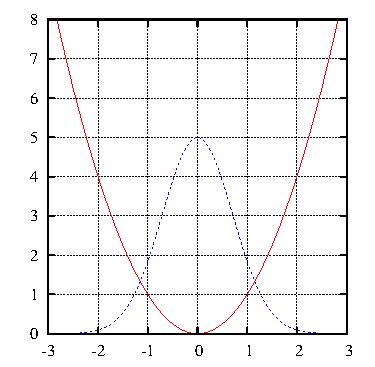
\includegraphics{image/harmonic.pdf}}
\end{frame}

%-*- coding:utf-8 -*-

\begin{frame}[t,fragile]{Metropolis法}
  \begin{itemize}
    %\setlength{\itemsep}{1em}
  \item 現在の配位$x$から、試行配位(trial configuration) $x'$を$x - \Delta \sim x + \Delta$の一様分布より選ぶ
  \item 確率$\min \Big( 1, \frac{e^{-\beta V(x')}}{e^{-\beta V(x)}} \Big)$で$x'$を採択(accept)。棄却(reject)された場合にはもとの$x$のまま
  \item 物理量の測定 (reject された場合にもカウントする)
  \item 採択確率(acceptance probability)は、$\frac{e^{-\beta V(x')}}{e^{-\beta V(x)}+e^{-\beta V(x')}}$でもよい
  \item 例: \href{https://github.com/todo-group/computer-experiments/blob/master/exercise/monte_carlo/harmonic.c}{harmonic.c}
  \end{itemize}
\end{frame}

\begin{frame}[t,fragile]{Metropolis法によるシミュレーション}
  \begin{itemize}
    \setlength{\itemsep}{1em}
  \item $\Delta = 0.1$
    
    \vspace*{-2em}\hfill \resizebox{9cm}{!}{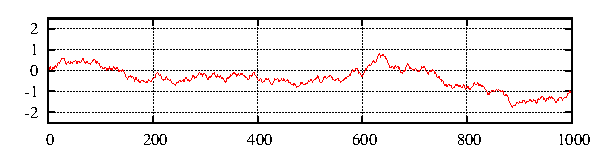
\includegraphics{image/series-001.pdf}}
  \item $\Delta = 1$
    
    \vspace*{-2em}\hfill \resizebox{9cm}{!}{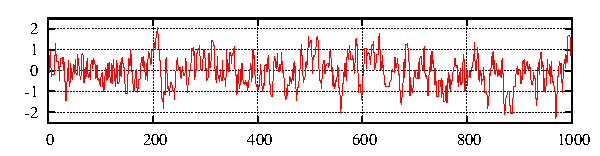
\includegraphics{image/series-010.pdf}}
  \item $\Delta = 10$
    
    \vspace*{-2em}\hfill \resizebox{9cm}{!}{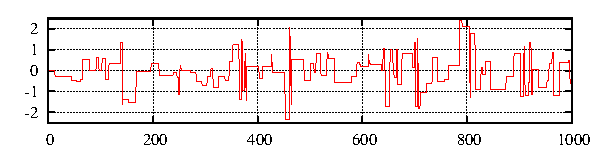
\includegraphics{image/series-100.pdf}}
  \end{itemize}
\end{frame}

%-*- coding:utf-8 -*-

\begin{frame}[t,fragile]{自己相関関数(autocorrelation function)}
  \begin{itemize}
    %\setlength{\itemsep}{1em}
  \item エルゴード性 + つりあい条件 ⇒ 原理的に正しいマルコフ連鎖モンテカルロ
  \item 実際には自己相関を考慮する必要あり
  \item 自己相関関数
    \[
    C(t) = \frac{\langle A_{i+t}A_i \rangle - \langle A \rangle^2}{\langle A^2 \rangle - \langle A \rangle^2} \sim \exp(-\frac{t}{\tau})
    \]
  \item $\tau$: 自己相関時間(autocorrelation time)
  \item 自己相関の影響により、統計的な「有効サンプル数」が減少
    \[
    M \rightarrow \frac{M}{1+2\tau}
    \]
  \end{itemize}
\end{frame}

\begin{frame}[t,fragile]{自己相関時間と統計誤差}
  \hspace*{4em} 自己相関時間 \hspace*{9em} 統計誤差

  \noindent\resizebox{0.49\textwidth}{!}{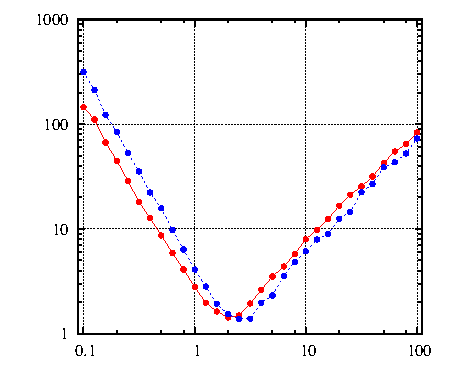
\includegraphics{image/autocorr.pdf}}
  \resizebox{0.49\textwidth}{!}{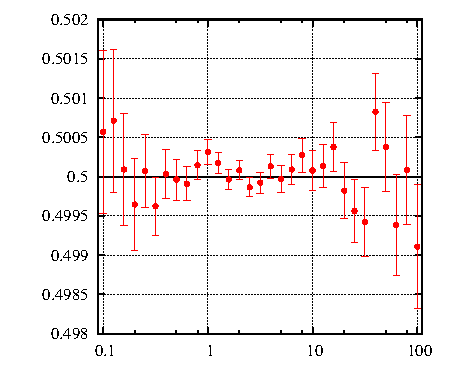
\includegraphics{image/error.pdf}}

  \hspace*{7em} $\Delta$ \hspace*{12em} $\Delta$
\end{frame}

\begin{frame}[t,fragile]{マルコフ連鎖モンテカルロ法}
  \begin{itemize}
    %\setlength{\itemsep}{1em}
  \item 統計誤差はサンプルの生の分散$s^2$とサンプル数$M$、自己相関時間$\tau$で決まる
    \[
    \sigma^2 \simeq \frac{s^2 (1+2\tau)}{M}
    \]
    \begin{itemize}
    \item 一度に大きく配位を動かそうとすると棄却率が増加 $\Rightarrow$ $\tau$が増加
    \item 動かす幅を小さくすると棄却率は高いが相関が消えない $\Rightarrow$ $\tau$が増加
    \item 非局所更新法、拡張アンサンブル法など様々な方法が使われている
    \end{itemize}
  \item 物理以外でも、Bayes推定や機械学習、社会現象のシミュレーションなど広く使われている
  \end{itemize}
\end{frame}

\begin{frame}[t,fragile]{イジング模型に対するモンテカルロ法}
  \begin{itemize}
    %\setlength{\itemsep}{1em}
  \item 更新の単位は一つのスピンとするのが一番自然
  \item メトロポリス法に必要なのは更新前後のエネルギー差だけなので、全エネルギーを計算しなおす必要なし
\begin{verbatim}
for (s = 0; s < num_sites; ++s) {
  delta = 0.0;
  for (j = 0; j < num_neighbors; ++j) {
    v = neighbor(s, j);
    delta += 2 * J * spin[s] * spin[v];
  }
  if (random() < exp(-beta * delta))
    spin[s] = -1 * spin[s];
}  
\end{verbatim}
  \end{itemize}
\end{frame}

\begin{frame}[t,fragile]{物理量の計算}
  \begin{itemize}
    %\setlength{\itemsep}{1em}
  \item 内部エネルギー$E$
    \begin{itemize}
    \item 初期状態のスピンを全て上向き(1)に取ると$E=-J \times \text{ボンド数}$
    \item モンテカルロステップ毎にエネルギーの変化分を計算しているので、採択された場合にはその値を足し込む
    \end{itemize}
  \item 比熱$C$: 内部エネルギーのゆらぎから計算できる
    \[
    C = \frac{1}{N} \frac{\partial E}{\partial T} = \frac{1}{NT^2} (\langle E^2 \rangle - \langle E \rangle^2)
    \]
  \item 磁化$m$: スピンの値の平均値 $m = \frac{1}{N} \sum_i \sigma_i$
    \begin{itemize}
    \item 外部磁場がない場合、対称性から$m$の長時間平均は厳密には零になる
    \item 熱力学極限では対称性が自発的に破れて、低温で有限の$m$
    \item シミュレーションでは$m$ではなく$m^2$を見るとよい
    \end{itemize}
  \end{itemize}
\end{frame}

%-*- coding:utf-8 -*-

\begin{frame}[t,fragile]{モンテカルロステップの設定}
  \begin{itemize}
    %\setlength{\itemsep}{1em}
  \item 全てのスピンについて一通り更新を試すのを、1モンテカルロステップと数える
  \item どれくらいのモンテカルロステップが必要かは、あらかじめは分からない
  \item 典型的には、$10^4$---$10^6$程度にとることが多い
  \item 熱平衡化 (thermalization)
    \begin{itemize}
    \item 初期配位依存性を取り除くため、モンテカルロステップの最初の部分は捨てる(burn-in time)
    \item 典型的には、全体の1割程度を捨てることが多い
    \end{itemize}
  \end{itemize}
\end{frame}


\section{}
\begin{frame}[t]{本日の課題}
  \begin{itemize}
    %\setlength{\itemsep}{1em}
  \item 実習
    \begin{itemize}
    \item 講義資料の中の {\tt square\_lattice.c}, {\tt harmonic.c}をコンパイル・実行。ソースコードの中身を確認 \\

      {\tt harmonic.c}中のパラメータ{\tt delta} (講義資料中の$\Delta$)を変えて、位置$x$の時系列の振る舞いがどう変わるか確認 \\
      
      サンプルコード一式: \href{https://github.com/todo-group/ComputerExperiments/releases/tag/2020a-computer2}{example-2-2.zip}
    \item 実習課題一覧\href{https://github.com/todo-group/ComputerExperiments/releases/tag/2020a-computer2}{exercise-2.pdf}から適宜選び実習
    \end{itemize}
  \item 質問はSlackの「\# 6\_モンテカルロ法」あるいは他の適当と思われるチャンネルで
  \item 次回講義(10/16)の前日までにITC-LMSのアンケート「作業レポートNo.2」に回答
  \end{itemize}
\end{frame}

\section{参考資料: 転送行列法}

\begin{frame}[t,fragile]{転送行列: 一次元イジング模型}
  \begin{itemize}
    \setlength{\itemsep}{1em}
  \item ハミルトニアン: $H = - \sum_i \sigma_i \sigma_{i+1}$
  \item 分配関数
    \[
    Z = \sum_{\sigma_1}\sum_{\sigma_2}\cdots\sum_{\sigma_L} e^{\beta \sigma_1 \sigma_2} e^{\beta \sigma_2 \sigma_3} \cdots e^{\beta \sigma_L \sigma_1}
    \]
    \begin{itemize}
    \item $e^{\beta \sigma_1 \sigma_2}$は4通りの値を持つ→$2\times2$行列$T_{\sigma_1 \sigma_2}$の形に書くと
      \begin{align*}
      \sum_{\sigma_2} e^{\beta \sigma_1 \sigma_2} e^{\beta \sigma_2 \sigma_3} &= \sum_{\sigma_2} T_{\sigma_1 \sigma_2} T_{\sigma_2 \sigma_3} = (T^2)_{\sigma_1 \sigma_3} \\
      Z &= {\rm tr} T^L
      \end{align*}
    \end{itemize}
  \end{itemize}
\end{frame}

\begin{frame}[t,fragile]{分配関数の計算方法}
  \begin{itemize}
    \setlength{\itemsep}{1em}
  \item ${\rm tr} T^L$の計算方法
    \begin{enumerate}
    \item $L$個の行列$T$を掛けて、最後にトレースを取る (行列・行列積)
    \item $(1,0)^t$と$(0,1)^t$にそれぞれ行列$T$を$L$回掛けて、それぞれの第1成分と第2成分を足し合わせる (行列・ベクトル積)
    \item 行列$T$を固有値分解: $T = U\Lambda U^{-1}$しておくと
      \[
        {\rm tr} T^L = {\rm tr} (U \Lambda U^{-1})^L = {\rm tr} U \Lambda^L U^{-1} = {\rm tr} \Lambda^L = \lambda_1^L + \lambda_2^L
        \]
        特に$|\lambda_1| > |\lambda_2|$とすると$L\rightarrow\infty$で
        \[
          {\rm tr} T^L \simeq \lambda_1^L
          \]
    \end{enumerate}
  \end{itemize}
\end{frame}

\begin{frame}[t,fragile]{二次元正方格子への拡張}
  \begin{itemize}
    \setlength{\itemsep}{1em}
  \item $L \times M$の正方格子
    \begin{itemize}
    \item 第$i$列のスピンをまとめて$s_i = ( \sigma_{i,1}, \sigma_{i,2}, \cdots, \sigma_{i,M})$とする
    \item $s_i$は$2^M$通りの値をとる
    \end{itemize}
  \item 転送行列
    \begin{itemize}
    \item 横方向の相互作用: $\exp[\beta \sum_j \sigma_{i,j} \sigma_{i+1,j}]$ \ ($2^M \times 2^M$の密行列)
    \item 縦方向の相互作用: $\exp[\beta \sum_j \sigma_{i,j} \sigma_{i,j+1}]$ \ ($2^M \times 2^M$の対角行列)
    \item それぞれ$U$, $D$と表すと
      \[
      Z = {\rm tr} \, DUDU \cdots DU
      \]
    \item さらに$T=D^{1/2}TD^{1/2}$と定義すると、$T$は対称行列となり
      \[
      Z = {\rm tr} \, T^L
      \]
    \end{itemize}
  \end{itemize}
\end{frame}

\begin{frame}[t,fragile]{計算コスト}
  \begin{itemize}
    \setlength{\itemsep}{1em}
  \item 必要メモリと必要計算量の見積もり
    \begin{enumerate}
    \item $L$個の行列$T$を掛けて、最後にトレースを取る \\
      メモリ〜$(2^M)^2$, 計算量〜$L(2^M)^3$
    \item $2^M$個の基底ベクトルにそれぞれ行列$T$を$L$回掛けて、それぞれの対応する成分を足し合わせる \\
      メモリ〜$(2^M)^2$, 計算量〜$L(2^M)^3$
    \item 行列$T$を固有値分解(Householder法) \\
      メモリ〜$(2^M)^2$, 計算量〜$(2^M)^3$
    \end{enumerate}
  \end{itemize}
\end{frame}

\begin{frame}[t,fragile]{疎行列分解}
  \begin{itemize}
    \setlength{\itemsep}{1em}
  \item 行列$U$は疎行列の積に分解できる: $U = U_1 U_2 \cdots U_M$ \\
    ここで
    \[
    (U_k)_{s_i, s_{i+1}} = \exp[\beta \sigma_{i,k} \sigma_{i+1,k}] \prod_{j \ne k} \delta_{\sigma_{i,j} \sigma_{i+1,j}}
    \]
    \begin{itemize}
    \item 各行各列に非零の要素は2つだけ
    \item $U_k$の要素はその場で簡単に計算できる(メモリコスト=0)
    \item ベクトルと行列$U_k$の積: 計算量〜$2 \times 2^M$
    \item 密行列と行列$U_k$の積: 計算量〜$2 \times (2^M)^2$
    \end{itemize}
  \end{itemize}
\end{frame}

\begin{frame}[t,fragile]{計算コスト再見積もり}
  \begin{itemize}
    \setlength{\itemsep}{1em}
  \item 必要メモリと必要計算量の見積もり
    \begin{enumerate}
    \item $L$個の行列$T$を掛けて、最後にトレースを取る \\
      メモリ〜$(2^M)^2$, 計算量〜$LM(2^M)^2$
    \item $2^M$個の基底ベクトルにそれぞれ行列$T$を$L$回掛けて、それぞれの対応する成分を足し合わせる \\
      メモリ〜$2^M$, 計算量〜$LM(2^M)^2$
    \item 行列$T$を固有値分解
      \begin{itemize}
        \item $L$有限の場合 \\
          メモリ〜$(2^M)^2$, 計算量〜$(2^M)^3$
        \item $L\rightarrow\infty$の極限: 最大固有値$\lambda_1$のみ必要 \\
          メモリ〜$2^M$, 計算量〜$O(100)\times M(2^M)$
      \end{itemize}
    \end{enumerate}
  \end{itemize}
\end{frame}


\end{document}
